\documentclass[12pt]{article}
\usepackage[pdftex]{graphicx}
\newcommand{\kg}{\mathrm{kg}}
\newcommand{\m}{\mathrm{m}}
\newcommand{\s}{\mathrm{s}}
\begin{document}
\newcounter{problem}
\thispagestyle{empty}

\section*{NYU General Physics 1---Problem set 3}

\paragraph{Problem~\theproblem:}\refstepcounter{problem}%
The Space Station orbits Earth in ``low earth orbit'' meaning that,
from a Solar-System perspective, it is just skimming over Earth's
surface in a circular orbit.

\textsl{(a)} Assume that the Space Station experiences the same
acceleration $g$ due to gravity as we do on the Earth's surface.  What
combination of $g$ and the Earth's radius $R$ can you make that has
units of time?  What combination has units of velocity?

\textsl{(b)} Now put the Space Station on a circular orbit, and assume
that the centripetal acceleration of that orbit is given by $g$.  What
is the orbital period $T$ and orbital speed $v$ in terms of $g$ and the
orbital radius $R$?

\textsl{(c)} Look up (on the internet, perhaps) the altitude of the
Space Station above the Earth's surface and look up the radius of the
Earth.  What is the fractional amount by which the Space Station is
further from the center of the Earth than we are here in New York?  Is
the assumption that the acceleration is $g$ reasonable?

\textsl{(d)} Look up the period of the Space Station's orbit.  Is your
calculation in part \textsl{(b)} correct?

\textsl{(e)} What does this problem have to do with a centrifuge, if
anything?

\paragraph{Problem~\theproblem:}\refstepcounter{problem}%
Two blocks on a stationary horizontal table are joined by a light,
inextensible string, as shown.  The rightmost block is pulled to the
right by a force of magnitude
$F$.\\ 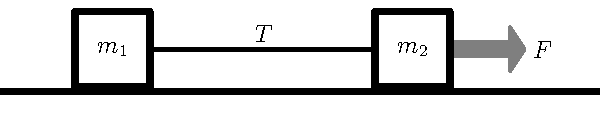
\includegraphics{../py/stringblocks.pdf}

\textsl{(a)} Draw free-body diagrams for both blocks, showing all
forces (and nothing else).

\textsl{(b)} What is the necessary relationship between the
acceleration $\vec{a}_1$ of block 1 and the acceleration $\vec{a}_2$
of block 2?

\textsl{(c)} What is the tension $T$ in the string and the
acceleration $a$ of the whole system?

\textsl{(d)} Why, exactly, do we treat the string as light?  Why as
inextensible?  How do these two approximations make the calculation
simpler?

\paragraph{Problem~\theproblem:}\refstepcounter{problem}%
A block of mass $m=7\,\kg$ lies on a horizontal table.  It is
stationary relative to the table.  Now imagine that the table is
accelerating upwards (in, say, an elevator) with an acceleration of magnitude
$0.9\,\m\,\s^{-2}$.  Draw a free body diagram for the block and
calculate the magnitude of the force on the block from the table.

\end{document}
